\documentclass{article}
\usepackage{graphicx}
\usepackage[utf8]{inputenc}
\usepackage[italian]{babel}
\usepackage[T1]{fontenc}
\usepackage{fancyhdr}
\usepackage{biblatex}
\usepackage{csquotes}

\addbibresource{biblio.bib}

\graphicspath{{./images/}}

\pagestyle{fancy}
\fancyhf{}
\lhead{Progetto finale di Reti Logiche}
\rhead{\leftmark}
\rfoot{\thepage}
\lfoot{}
\renewcommand{\headrulewidth}{0.5pt}
\renewcommand{\footrulewidth}{0.5pt}

% add only section and subsection to the index
\addtocontents{toc}{\protect\setcounter{tocdepth}{2}}
% needed for the index
\makeindex
% removed ident space for paragraph
\setlength{\parindent}{0pt}

\begin{document}

\begin{titlepage}
    \centering
    \vspace*{\fill}
    \Huge\textbf{Progetto finale di \\ Reti Logiche}\\
    \vspace{5mm} %5mm vertical space
    \Large Prof. Gianluca Palermo - Anno di corso 2020-21\\
    \vspace{5mm} %5mm vertical space
    \large Francesco Pastore - Codice persona: 10629332\\
    \vspace{100mm}
    \vspace*{\fill}
\end{titlepage}

\thispagestyle{empty}
\tableofcontents
\pagebreak

\section{Introduzione}
Il progetto richiede l'implementazione in VHDL dell'algoritmo di equalizzazione dell'istogramma di un'immagine. Questo metodo di elaborazione permette di aumentare il contrasto di un'immagine andando a distribuire su tutto lo spetttro, in modo bilanciato, i valori di intensità precedentemente vicini. In particolare viene richiesta l'implementazione di una versione semplificata applicata solo ad immagini in scala di grigi (0-255) e grandi al massimo 128x128 pixel.
\begin{figure}[h]
    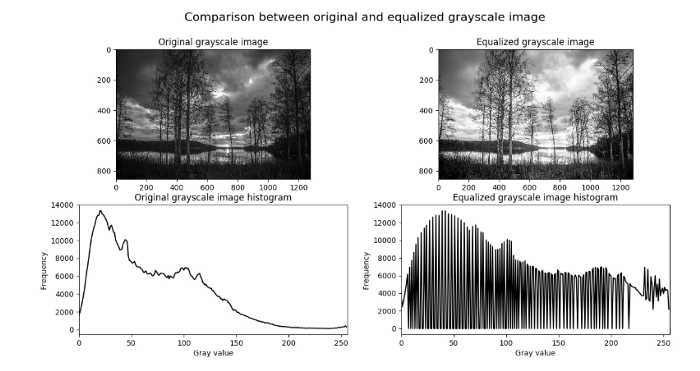
\includegraphics[scale=0.25]{equalization.png}
    \centering
    \caption{Esempio di equalizzazione dell'istogramma di un'immagine. \cite{equalization}}
\end{figure}

\subsection{Specifiche di progetto}
L'interfaccia del componente è stata definita nella specifica con i relativi segnali di ingresso e di uscita. Oltre a questo, è stata definita la struttura della memoria e l'indirizzamento dei dati. All'indirizzo zero è possibile trovare il numero di colonne, seguito all'indirizzo uno da quello di righe. Dall'indirizzo due iniziano invece i valori dei singoli pixel dell'immagine fino alla posizione NUM\_COLS * NUM\_ROWS + 1. La scrittura dei pixel equalizzati deve avvenire invece dall'indirizzo immediatamente successivo all'ultimo pixel dell'immagine.
\begin{figure}[h]
    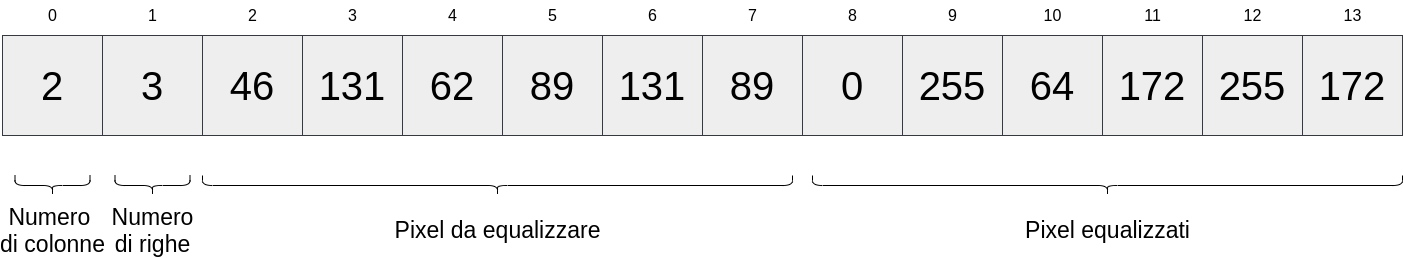
\includegraphics[width=\textwidth]{memory.png}
    \centering
    \caption{Dettaglio della struttura della memoria ed esempio di equalizzazione}
\end{figure}

\pagebreak

\subsection{Algoritmo in breve}
Di seguito una breve descrizione dei punti principali dell'algoritmo da implementare. Fare riferimento alle formule per il calcolo dei valori considerati.
\begin{enumerate}
    \item Lettura del numero di colonne.
    \item Lettura del numero di righe.
    \item Verificare che l'immagine non sia vuota, altrimenti terminare l'esecuzione.
    \item Lettura dei pixel dell'immagine cercando il valore minimo e massimo.
    \item Calcolare il delta\_value e il relativo shift\_level.
    \item Seconda lettura dell'immagine con equalizzazione dei pixel.
    \item Scrittura in memoria dei nuovi valori dei pixel.
\end{enumerate}
\begin{figure}[h]
    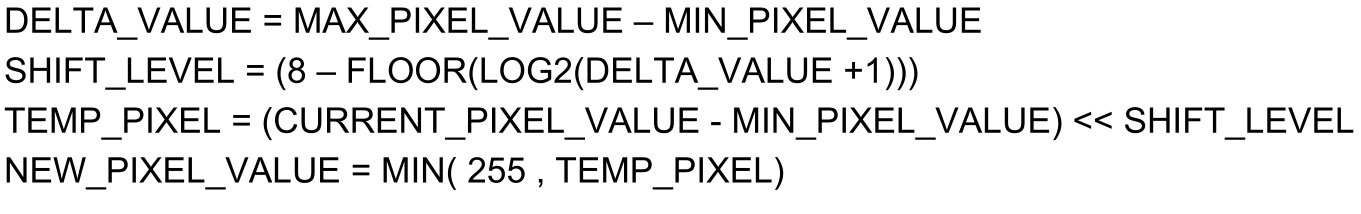
\includegraphics[width=\textwidth]{formulas.png}
    \centering
    \caption{Formule dell'algoritmo di equalizzazione fornite nella specifica.}
\end{figure}

\subsection{Note di implementazione}
Rispetto all'algoritmo descritto in precedenza, l'implementazione in VHDL richiede alcune modifiche.
\begin{itemize}
    \item La lettura dalla memoria non è istantanea, ma necessita di un ciclo di clock di attesa dopo aver effettuato la richiesta. In particolare nel componente è stato implementato lo stato MEM\_WAIT.
    \item L'assegnamento di valori ai segnali non è immediato, ma avviene al ciclo di clock successivo. Per questo motivo alcune operazioni vengono eseguite in stati successivi.
    \item Non è possibile assegnare ad un segnale esso stesso neppure con modifiche. Questo richiede, ad esempio per il contatore, di utilizzare un altro segnale come appoggio per effettuare l'incremento.
\end{itemize}

\pagebreak

% ------ ARCHITETTURA -----
\section{Architettura}
\subsection{Segnali utilizzati}

\subsubsection{num\_cols, num\_pixels, count e tmp\_count}
Per eseguire la lettura dell'immagine è necessario conoscere la dimensione, sfruttando il numero di colonne e di righe e un relativo contatore. In VHDL non essendo possibile assegnare un segnale a se stesso, è stato necessario aggiungere un contatore d'appoggio tmp\_count. Il range di count, temp\_count e num\_pixels è pari a 0-16384 perchè ogni immagine può essere grande al massimo 128x128.

\subsubsection{min\_pixel\_value e max\_pixel\_value}
Questi segnali contengono, dopo la prima lettura dell'immagine, il valore del pixel massimo e minimo necessari per il calcolo delle varie formule di equalizzazione. Sono stati dichiarati di tipo INTEGER con range 0-255 perchè su di essi vengono effettuare diverse operazioni aritmetiche e logiche.

\subsubsection{state\_next, state\_after\_wait e state\_after\_read}
Per le transizioni tra i vari stati sono stati defini alcuni segnali che contengono gli stati prossimi. Di specifico state\_next contiene sempre lo stato immediatamente successivo, state\_after\_wait il seguente a MEM\_WAIT mentre state\_after\_read lo stato successivo a READ\_PIXEL.

\begin{figure}[h]
    \vspace{1cm}
    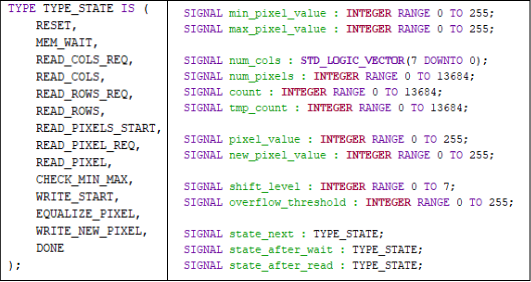
\includegraphics[width=\textwidth]{signals-definition.png}
    \centering
    \caption{Dichiarazione dei segnali utilizzati e del tipo TYPE\_STATE}
\end{figure}

\pagebreak

\subsubsection{shift\_level e overflow\_threshold}
Dopo aver calcolato minimo e massimo è possibile determinare il valore del delta\_value e del relativo shift\_level. In particolare oltre a questo valore è stato aggiunta anche la soglia di overflow utile per controllare il valore da equalizzare prima di effettuare lo shift. Lo shift\_level è da definizione un valore intero compreso tra 0 e 8, mentre il delta\_value e l'overflow\_threshold contengono valori di pixel quindi appartengono al range 0-255.


\subsubsection{pixel\_value e new\_pixel\_value}
Entrambi questi segnali contengono valori di pixel dell'immagine e su di essi vengono effettuate diverse operazioni, per questo motivo sono di tipo INTEGER con range 0-255. In particolare pixel\_value contiene il valore di ciascun pixel letto mentre il new\_pixel\_value serve come appoggio per il calcolo del pixel equalizzato.

\subsection{Esempio di utilizzo dei segnali}
Per mostrare l'utilizzo effettivo dei segnali, qui di seguito è presente una possibile applicazione con il caso di esempio proposto per la struttura della memoria.

\begin{figure}[h]
    \vspace{1cm}
    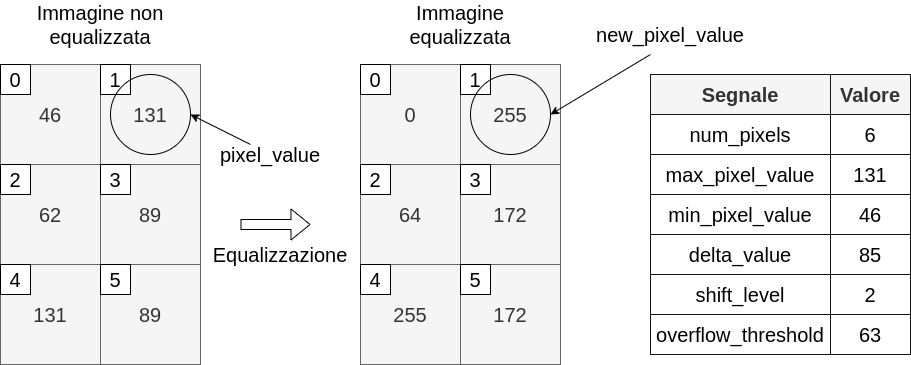
\includegraphics[width=\textwidth]{example.png}
    \centering
    \caption{Esempio di equalizzazione di un'immagine con relativi valori dei segnali fondamentali}
\end{figure}

\pagebreak

\subsection{Descrizione degli stati}
Il modulo è stato realizzato come una macchina a stati, in particolare comprende 14 stati descritti di seguito.

\subsubsection{RESET}
Lo stato di RESET è lo stato iniziale della macchina ed è l'unico raggiungibile da tutti gli altri. Quando il componente riceve un segnale di i\_rst alto ferma l'esecuzione per poi ripartire dallo stato di reset. La macchina esce da questo stato solo con il segnale i\_start alto.

\subsubsection{READ\_COLS\_REQ}
Nel primo byte della memoria è salvato il numero di colonne dell'immagine. Questo stato si occupa di effettuare la relativa richiesta di lettura. Essendo una lettura è necessario attendere che la memoria elabori la richiesta, per questo motivo lo stato successivo è MEM\_WAIT.

\subsubsection{READ\_COLS}
Dopo aver effettuato la richiesta di lettura nello stato READ\_COLS\_REQ in questo stato la macchina legge il numero di colonne passatole dalla memoria nel bus i\_data.

\subsubsection{READ\_ROWS\_REQ}
Il secondo elemento in memoria dopo il numero di colonne è il numero di righe. Anche in questo caso è necessario effettuare la richiesta di lettura, aspettare un ciclo di clock nello stato MEM\_WAIT e solo dopo leggere il valore richiesto.

\subsubsection{READ\_ROWS}
Dopo aver effettuato la richiesta di lettura in READ\_ROWS\_REQ e aspettato per l'elaborazione da parte della memoria in MEM\_WAIT in questo stato viene letto il numero di righe passato al componente tramite i\_data. In questo caso viene calcolato direttamente il numero di pixel che costituiscono l'immagine moltiplicando il valore ricevuto per il numero di colonne richiesto in precedenza.

\subsubsection{READ\_PIXELS\_START}
In questo stato viene inizializzato il contatore  e i segnali di minimo e massimo prima di effettuare la prima scansione dell'immagine. Il minimo viene settato a 255 che corrisponde al più alto valore possibile, il massimo invece a zero che rappresenta rispettivamente quello più basso. Viene controllato inoltre che non sia stata data un'immagine vuota, altrimenti si passa direttamente allo stato di DONE.

\subsubsection{READ\_PIXEL\_REQ}
Dopo aver calcolato il numero di pixel contenuti nell'immagine grazie al numero di colonne e di righe, è possibile leggerli scansionandola dall'inizio alla fine. In questo stato viene quindi settato l'indirizzo per la lettura del prossimo pixel che verrà poi letto nello stato READ\_NEXT\_PIXEL. Il contatore necessario per la lettura viene incrementato in questo stato sfruttando un segnale temporaneo d'appoggio.

\subsubsection{READ\_PIXEL}
Dopo aver effettuato la richiesta di lettura e aspettato l'elaborazione da parte della memoria, in questo stato la macchina legge il pixel passatole nell'ingresso i\_data. Viene inoltre salvato il valore del contatore, che era stato incrementato nello stato precedente sfruttando un segnale d'appoggio.

\subsubsection{MEM\_WAIT}
La memoria richiede un ciclo di clock per l'elaborazione di una richiesta di lettura. Questo stato serve quindi come attesa dopo aver settato o\_addr e o\_en.

\subsubsection{CHECK\_MIN\_MAX}
La prima scansione serve per trovare i valori minimi e massimi dei pixel dell'immagine, in modo da poter poi effettuare l'equalizzazione. In questo stato viene quindi controllato ciascun pixel dopo la prima lettura e confrontato con i valori di massimo e minimo temporanei.

\subsubsection{WRITE\_START}
Una volta effettuata la prima scansione e aver trovato quindi il massimo e il minimo, è possibile calcolare il delta\_value dato dalla differenza dei due valori. Tramite uno switch e le relative soglie, viene determinato lo shift\_level e il relativo overflow\_threshold. Per poter effettuare la seconda scansione, in questo stato viene inizializzato nuovamente il contatore.

\subsubsection{EQUALIZE\_PIXEL}
Per evitare di effettuare più volte lo stesso calcolo, in questo stato viene salvata nel segnale new\_pixel\_value la differenza tra il valore di ciascun pixel e il relativo minimo dopo ogni lettura.

\subsubsection{WRITE\_NEW\_PIXEL}
È in questo stato che la macchina scrive il valore del pixel equalizzato facendo attenzione ad effettuare lo shift solo quando non c'è overflow. A questo fine viene sfruttato il valore di soglia definito nello stato WRITE\_START sulla base del delta\_value.

\subsubsection{DONE}
È lo stato finale in cui giunge la macchina al termine di un'esecuzione completa. Viene settato o\_done ad alto e si rimane in attesa che venga abbassato il segnale di i\_start come da specifica. Una volta ricevuto quest'ultimo valore, si passa allo stato di RESET in modo da prepararsi ad un'altra possibile elaborazione.

\subsection{Diagramma degli stati}
\begin{figure}[h]
    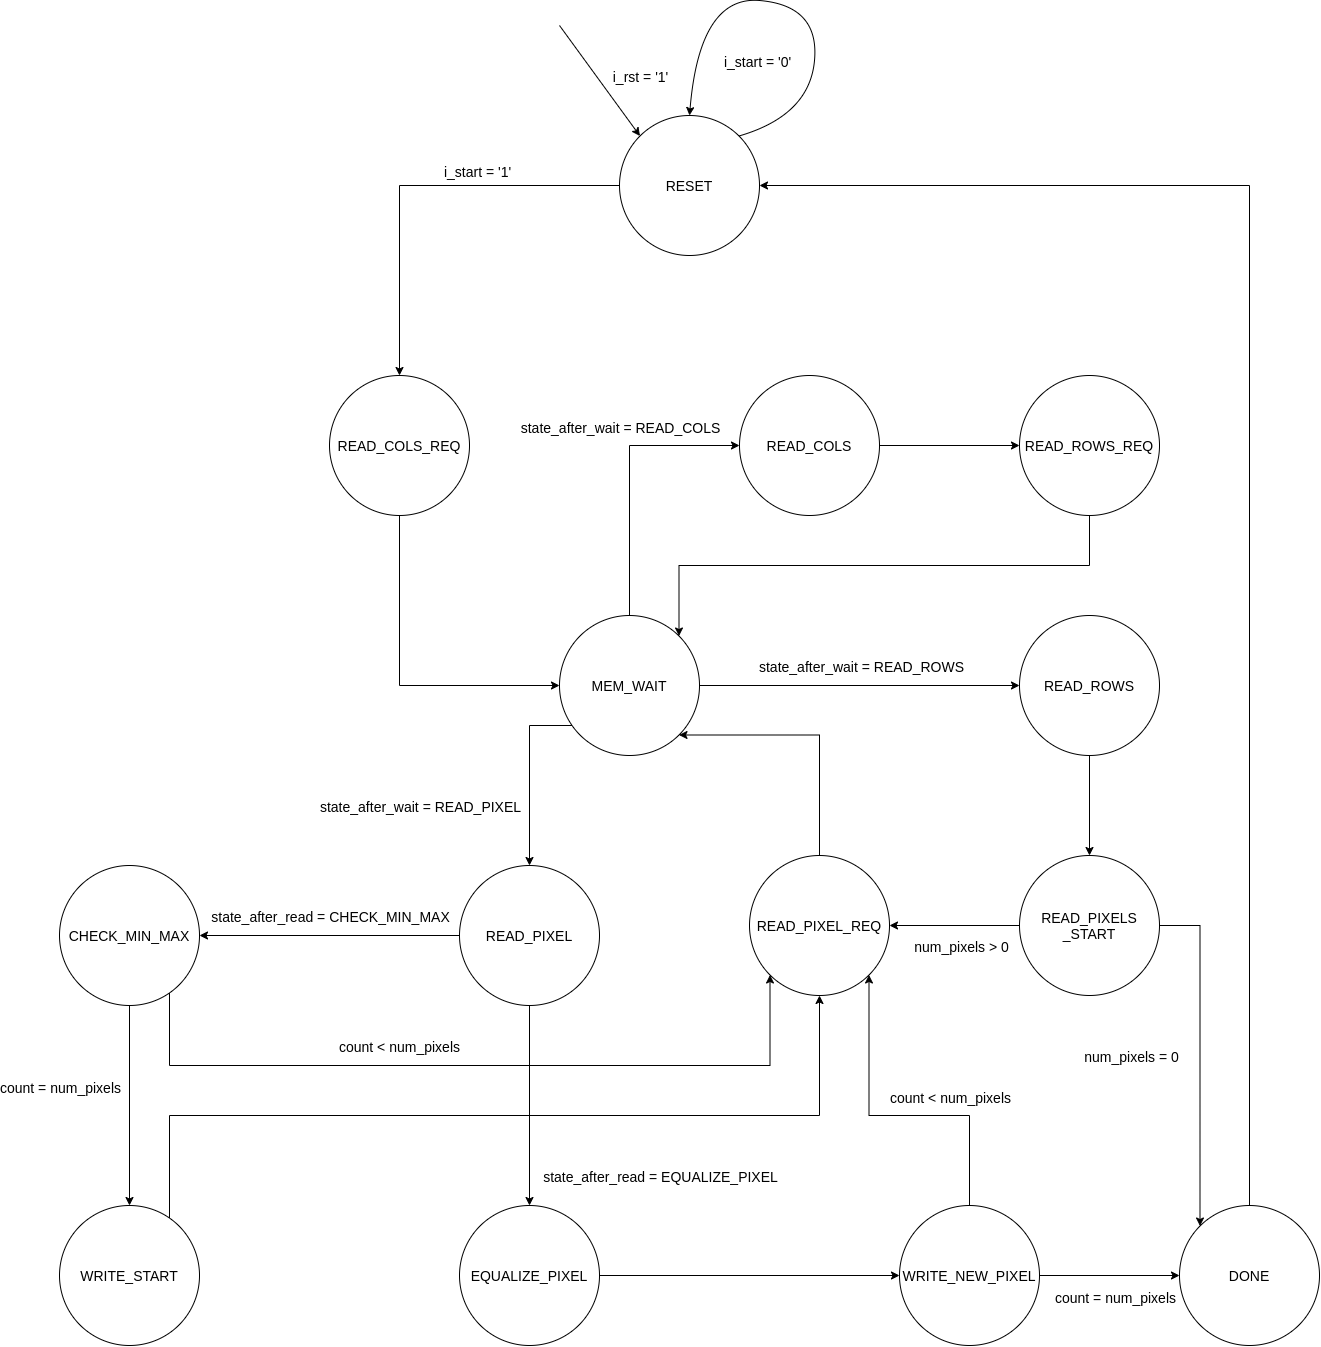
\includegraphics[width=\textwidth]{diagram.png}
    \centering
    \caption{Diagramma della macchina a stati, in figura sono state specificate le condizioni di transizione principali.}
\end{figure}

\pagebreak

% ------ RISULTATI SPERIMENTALI -----
\section{Risultati sperimentali}
\subsection{Simulazioni significative}
\subsubsection{Simulazione standard}
In questa simulazione è stato effettuato un test in una situazione standard. Da notare l'inizio dell'esecuzione solo dopo aver ricevuto il segnale di reset alto, poi abbassato e seguito da un segnale di start alto.
\begin{figure}[h]
    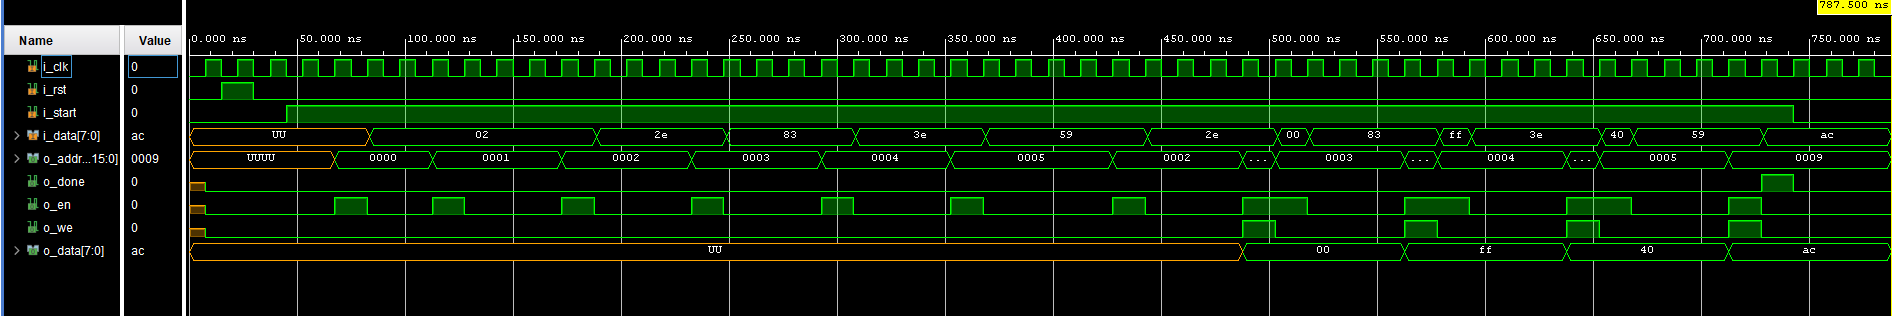
\includegraphics[width=\textwidth]{test-standard.png}
    \centering
    \caption{Simulazione standard}
\end{figure}

\subsubsection{Simulazione con immagine vuota}
Si può vedere come nel caso di un'immagine vuota, dopo aver letto il numero di colonne e quello di righe, la macchina termini immediatamente l'esecuzione. Da notare che il segnale di enable viene alzato soltanto due volte, appunto quelle necessarie per leggere solo le dimensioni.
\begin{figure}[h]
    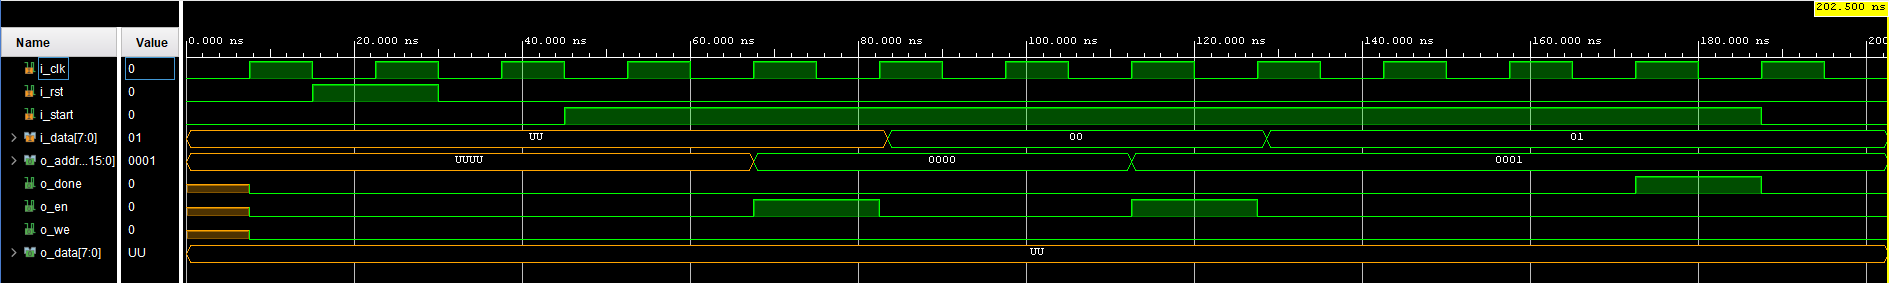
\includegraphics[width=\textwidth]{test-empty-image.png}
    \centering
    \caption{Simulazione con immagine vuota}
\end{figure}

\subsubsection{Simulazione con segnale di start ritardato}
Il componente prima di iniziare l'elaborazione deve attendere da specifica il segnale di start ad alto. È possibile vedere nell'immagine che esso rispetta correttamente l'attesa.
\begin{figure}[h]
    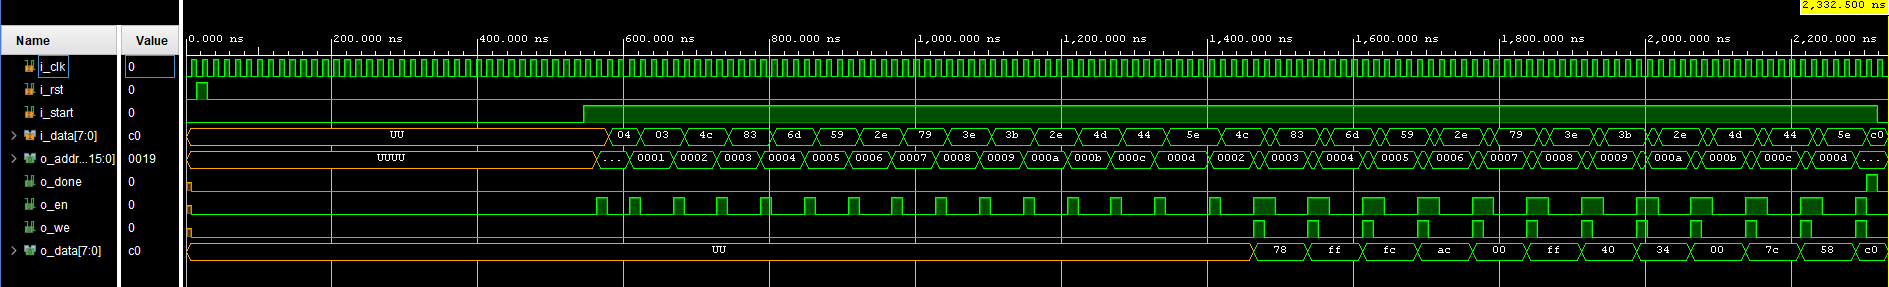
\includegraphics[width=\textwidth]{test-delayed-start.png}
    \centering
    \caption{Simulazione con segnale di start ritardato}
\end{figure}


\subsubsection{Simulazione con reset asincrono}
Tra le specifiche di progetto è presente la richiesta che la macchina possa essere resettata in qualsiasi momento, per poi reiniziare una nuova elaborazione. Da notare quindi nell'immagine che dopo aver ricevuto il segnale di reset, la macchina termini l'esecuzione per poi riprenderla una volta letto un segnale di start alto.
\begin{figure}[h]
    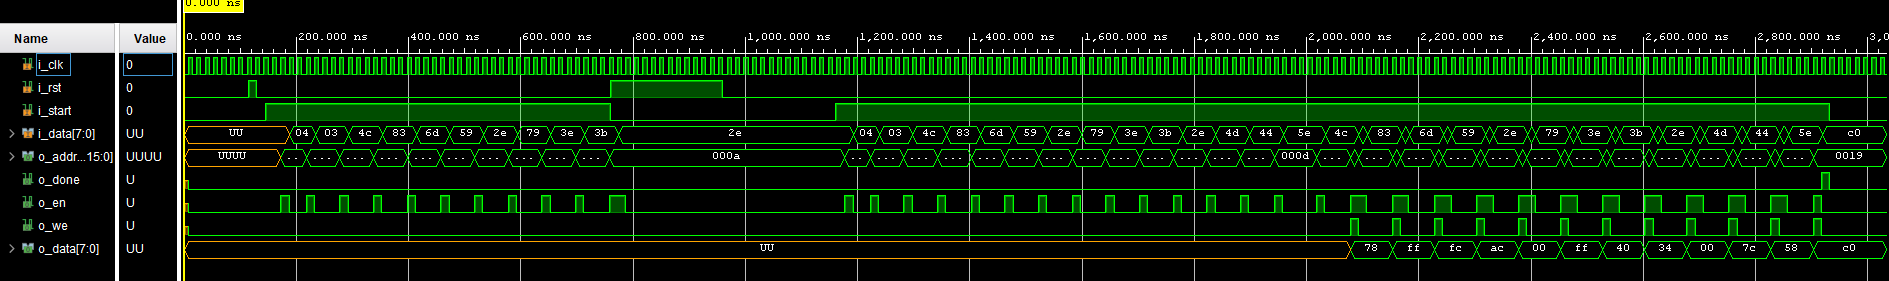
\includegraphics[width=\textwidth]{test-async-reset.png}
    \centering
    \caption{Simulazione con reset asincrono}
\end{figure}

\subsubsection{Simulazione con immagini multiple}
In questa simulazione si è testato l'elaborazione di immagini multiple controllando che la macchina rispetti correttamente il protocollo specificato. E possibile notare infatti che la macchina attende che il segnale di start venga alzato nuovamente prima di iniziare una nuova elaborazione. In particolare non è necessario un segnale di reset per far partire la nuova elaborazione.
\begin{figure}[h]
    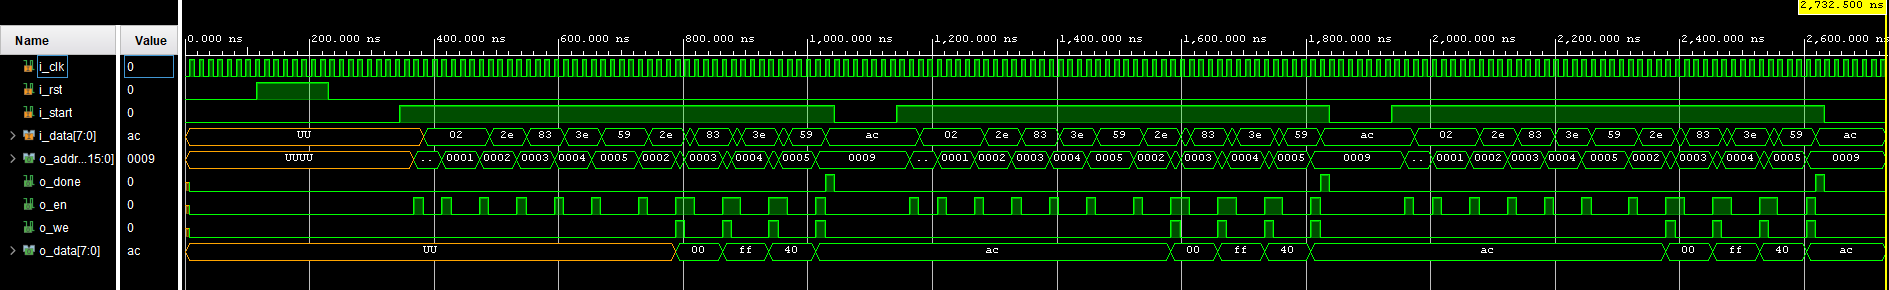
\includegraphics[width=\textwidth]{test-multiple-images.png}
    \centering
    \caption{Simulazione con immagini multiple}
\end{figure}

\subsubsection{Altre simulazioni}
Oltre alle simulazioni riportate, sono stati scritti altri testbench per effettuare ulteriori controlli di correttezza.
\begin{itemize}
    \item Simulazioni per controllare il calcolo di tutti i diversi delta\_value e relativi shift\_level, con verifica che venga gestito correttamente lo shift.
    \item Immagini con pixel tutti dello stesso valore, in questo caso il delta\_value è pari a zero e anche i new\_pixel\_value saranno a loro volta nulli.
    \item Immagini contenenti pixel con valori già spalmati su tutto il range 0-255. In questo caso dovranno essere riscritti gli stessi identici valori dato che lo shift\_level è pari a zero.
\end{itemize}

\pagebreak

\subsection{Report di sintesi}
Di seguito è possibile visionare i principali risultati della sintesi del componente. Rispetto al report di utilizzo l'elevato numero di LUT e FF è dovuto principalmente alla moltiplicazione per il calcolo del numero di pixel e allo shift per l'equalizzazione dei pixel. Entrambe però sono operazioni fondamentali per la risoluzione dell'algoritmo e non sono stati trovati altri modi per ottimizzarle.

\begin{figure}[h]
    \vspace{0.1cm}
    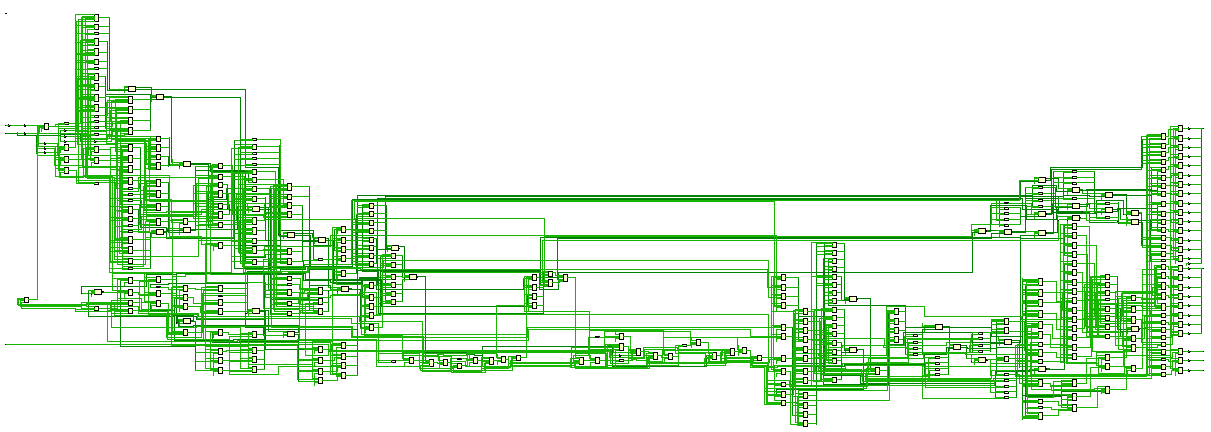
\includegraphics[width=\textwidth]{schema.png}
    \centering
    \caption{Schema del componente sintetizzato.}
\end{figure}

\begin{figure}[h]
    \vspace{0.4cm}
    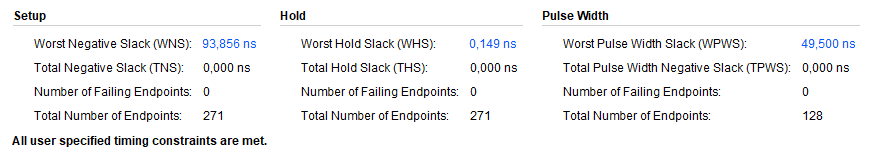
\includegraphics[width=\textwidth]{timing.png}
    \centering
    \caption{Riassunto del report di timing}
\end{figure}

\begin{figure}[h]
    \vspace{0.4cm}
    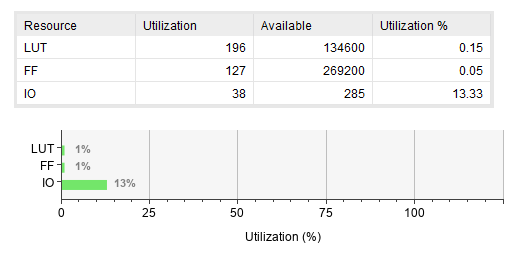
\includegraphics[scale=0.5]{utilization.png}
    \centering
    \caption{Riassunto del report di utilizzo}
\end{figure}

\pagebreak

\section{Conclusioni}
Il componente passa correttamente i test mostrati sia in behavioural che in post sintesi rispettando, almeno per i casi proposti, i requisiti della specifica. Sono stati scritti anche altri testbench per verificare il funzionamento in situazioni diverse e nei rispettivi casi limite. Per evitare di effettuare lo shift su 16 bit e poi controllarne il risultato, è stata implementata una soglia di overflow. In questo modo basta eseguire un confronto su 8 bit prima di shiftare il valore di new\_pixel\_value. Le operazioni di moltiplicazione e il calcolo di shift sono quelle più onerose, ma non è stato possibile trovare soluzioni alternative. Maggiori ottimizzazioni si potrebbero quindi effettuare trovando metodi migliori e meno onerosi di risorse.

\printbibliography

\end{document}